\documentclass[twoside]{book}

% Packages required by doxygen
\usepackage{fixltx2e}
\usepackage{calc}
\usepackage{doxygen}
\usepackage[export]{adjustbox} % also loads graphicx
\usepackage{graphicx}
\usepackage[utf8]{inputenc}
\usepackage{makeidx}
\usepackage{multicol}
\usepackage{multirow}
\PassOptionsToPackage{warn}{textcomp}
\usepackage{textcomp}
\usepackage[nointegrals]{wasysym}
\usepackage[table]{xcolor}

% Font selection
\usepackage[T1]{fontenc}
\usepackage[scaled=.90]{helvet}
\usepackage{courier}
\usepackage{amssymb}
\usepackage{sectsty}
\renewcommand{\familydefault}{\sfdefault}
\allsectionsfont{%
  \fontseries{bc}\selectfont%
  \color{darkgray}%
}
\renewcommand{\DoxyLabelFont}{%
  \fontseries{bc}\selectfont%
  \color{darkgray}%
}
\newcommand{\+}{\discretionary{\mbox{\scriptsize$\hookleftarrow$}}{}{}}

% Page & text layout
\usepackage{geometry}
\geometry{%
  a4paper,%
  top=2.5cm,%
  bottom=2.5cm,%
  left=2.5cm,%
  right=2.5cm%
}
\tolerance=750
\hfuzz=15pt
\hbadness=750
\setlength{\emergencystretch}{15pt}
\setlength{\parindent}{0cm}
\setlength{\parskip}{3ex plus 2ex minus 2ex}
\makeatletter
\renewcommand{\paragraph}{%
  \@startsection{paragraph}{4}{0ex}{-1.0ex}{1.0ex}{%
    \normalfont\normalsize\bfseries\SS@parafont%
  }%
}
\renewcommand{\subparagraph}{%
  \@startsection{subparagraph}{5}{0ex}{-1.0ex}{1.0ex}{%
    \normalfont\normalsize\bfseries\SS@subparafont%
  }%
}
\makeatother

% Headers & footers
\usepackage{fancyhdr}
\pagestyle{fancyplain}
\fancyhead[LE]{\fancyplain{}{\bfseries\thepage}}
\fancyhead[CE]{\fancyplain{}{}}
\fancyhead[RE]{\fancyplain{}{\bfseries\leftmark}}
\fancyhead[LO]{\fancyplain{}{\bfseries\rightmark}}
\fancyhead[CO]{\fancyplain{}{}}
\fancyhead[RO]{\fancyplain{}{\bfseries\thepage}}
\fancyfoot[LE]{\fancyplain{}{}}
\fancyfoot[CE]{\fancyplain{}{}}
\fancyfoot[RE]{\fancyplain{}{\bfseries\scriptsize Generated by Doxygen }}
\fancyfoot[LO]{\fancyplain{}{\bfseries\scriptsize Generated by Doxygen }}
\fancyfoot[CO]{\fancyplain{}{}}
\fancyfoot[RO]{\fancyplain{}{}}
\renewcommand{\footrulewidth}{0.4pt}
\renewcommand{\chaptermark}[1]{%
  \markboth{#1}{}%
}
\renewcommand{\sectionmark}[1]{%
  \markright{\thesection\ #1}%
}

% Indices & bibliography
\usepackage{natbib}
\usepackage[titles]{tocloft}
\setcounter{tocdepth}{3}
\setcounter{secnumdepth}{5}
\makeindex

% Hyperlinks (required, but should be loaded last)
\usepackage{ifpdf}
\ifpdf
  \usepackage[pdftex,pagebackref=true]{hyperref}
\else
  \usepackage[ps2pdf,pagebackref=true]{hyperref}
\fi
\hypersetup{%
  colorlinks=true,%
  linkcolor=blue,%
  citecolor=blue,%
  unicode%
}

% Custom commands
\newcommand{\clearemptydoublepage}{%
  \newpage{\pagestyle{empty}\cleardoublepage}%
}

\usepackage{caption}
\captionsetup{labelsep=space,justification=centering,font={bf},singlelinecheck=off,skip=4pt,position=top}

%===== C O N T E N T S =====

\begin{document}

% Titlepage & ToC
\hypersetup{pageanchor=false,
             bookmarksnumbered=true,
             pdfencoding=unicode
            }
\pagenumbering{alph}
\begin{titlepage}
\vspace*{7cm}
\begin{center}%
{\Large My Project }\\
\vspace*{1cm}
{\large Generated by Doxygen 1.8.14}\\
\end{center}
\end{titlepage}
\clearemptydoublepage
\pagenumbering{roman}
\tableofcontents
\clearemptydoublepage
\pagenumbering{arabic}
\hypersetup{pageanchor=true}

%--- Begin generated contents ---
\chapter{Hierarchical Index}
\section{Class Hierarchy}
This inheritance list is sorted roughly, but not completely, alphabetically\+:\begin{DoxyCompactList}
\item \contentsline{section}{Library\+:\+:I\+Account}{\pageref{class_library_1_1_i_account}}{}
\begin{DoxyCompactList}
\item \contentsline{section}{Library\+:\+:Bank\+Account}{\pageref{class_library_1_1_bank_account}}{}
\end{DoxyCompactList}
\end{DoxyCompactList}

\chapter{Class Index}
\section{Class List}
Here are the classes, structs, unions and interfaces with brief descriptions\+:\begin{DoxyCompactList}
\item\contentsline{section}{\mbox{\hyperlink{class_library_1_1_bank_account}{Library\+::\+Bank\+Account}} }{\pageref{class_library_1_1_bank_account}}{}
\item\contentsline{section}{\mbox{\hyperlink{class_library_1_1_i_account}{Library\+::\+I\+Account}} }{\pageref{class_library_1_1_i_account}}{}
\end{DoxyCompactList}

\chapter{Class Documentation}
\hypertarget{class_library_1_1_bank_account}{}\section{Library\+:\+:Bank\+Account Class Reference}
\label{class_library_1_1_bank_account}\index{Library\+::\+Bank\+Account@{Library\+::\+Bank\+Account}}
Inheritance diagram for Library\+:\+:Bank\+Account\+:\begin{figure}[H]
\begin{center}
\leavevmode
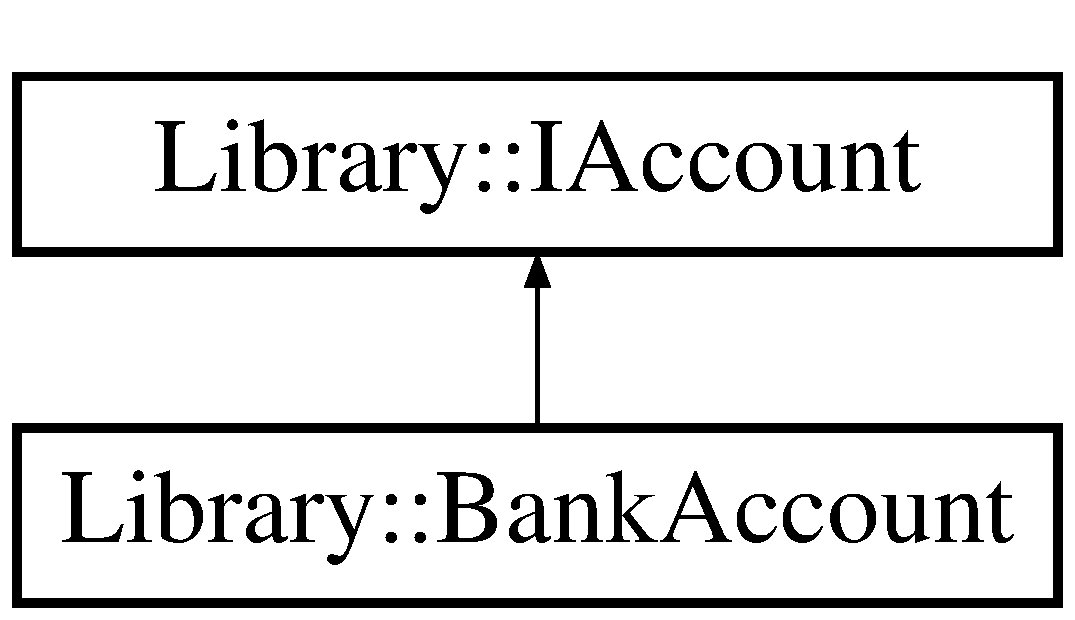
\includegraphics[height=2.000000cm]{class_library_1_1_bank_account}
\end{center}
\end{figure}
\subsection*{Public Member Functions}
\begin{DoxyCompactItemize}
\item 
\mbox{\Hypertarget{class_library_1_1_bank_account_a7e976ec5a3e0215352a848dc507ecedc}\label{class_library_1_1_bank_account_a7e976ec5a3e0215352a848dc507ecedc}} 
{\bfseries Bank\+Account} (double initial\+Balance=0)
\item 
\mbox{\Hypertarget{class_library_1_1_bank_account_a3976686819656beef170b3a8141cc056}\label{class_library_1_1_bank_account_a3976686819656beef170b3a8141cc056}} 
double {\bfseries check\+Balance} () const
\item 
\mbox{\Hypertarget{class_library_1_1_bank_account_afb2359035a3f9adc6ea2f22d05e28ac3}\label{class_library_1_1_bank_account_afb2359035a3f9adc6ea2f22d05e28ac3}} 
int {\bfseries deposit} (double amount)
\item 
\mbox{\Hypertarget{class_library_1_1_bank_account_a023fb06df2bcf499fa24209995b665c5}\label{class_library_1_1_bank_account_a023fb06df2bcf499fa24209995b665c5}} 
int {\bfseries withdraw} (double amount)
\end{DoxyCompactItemize}


The documentation for this class was generated from the following files\+:\begin{DoxyCompactItemize}
\item 
/\+Users/\+Bomb/\+Documents/\+Project/\+Learn-\/\+Cmake/\+Basics/\+Project-\/9/\+Library/include/account.\+hpp\item 
/\+Users/\+Bomb/\+Documents/\+Project/\+Learn-\/\+Cmake/\+Basics/\+Project-\/9/\+Library/src/account.\+cpp\end{DoxyCompactItemize}

\hypertarget{class_library_1_1_i_account}{}\section{Library\+:\+:I\+Account Class Reference}
\label{class_library_1_1_i_account}\index{Library\+::\+I\+Account@{Library\+::\+I\+Account}}
Inheritance diagram for Library\+:\+:I\+Account\+:\begin{figure}[H]
\begin{center}
\leavevmode
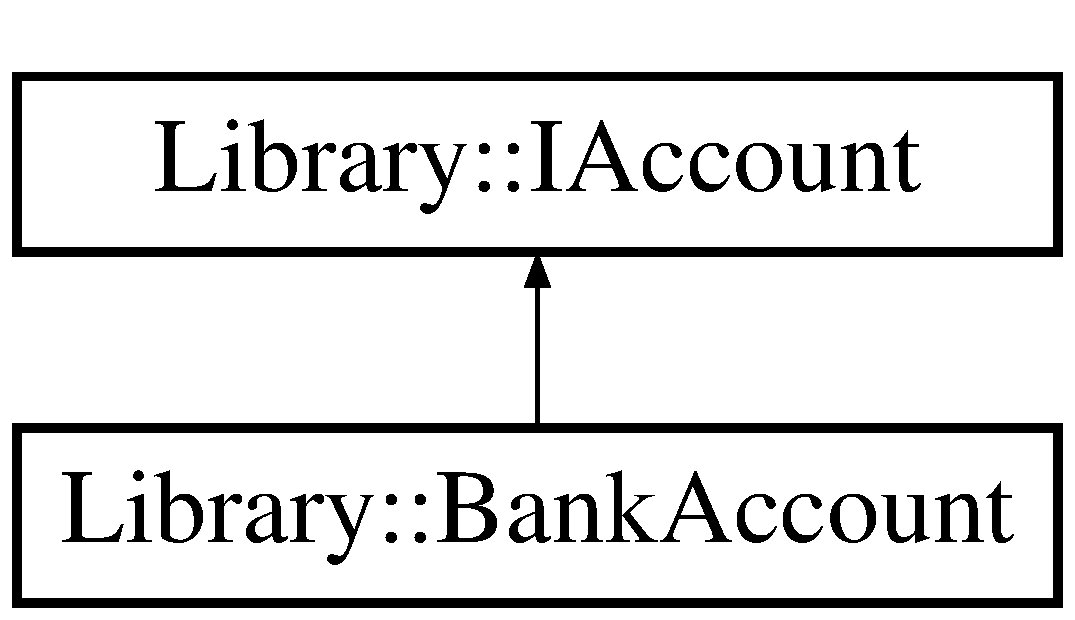
\includegraphics[height=2.000000cm]{class_library_1_1_i_account}
\end{center}
\end{figure}
\subsection*{Public Member Functions}
\begin{DoxyCompactItemize}
\item 
\mbox{\Hypertarget{class_library_1_1_i_account_a3eb1e12ae7fa2546e235a4a6c39e98f7}\label{class_library_1_1_i_account_a3eb1e12ae7fa2546e235a4a6c39e98f7}} 
virtual double {\bfseries check\+Balance} () const =0
\item 
\mbox{\Hypertarget{class_library_1_1_i_account_a4697c7630dd8868076155bd4acf313ff}\label{class_library_1_1_i_account_a4697c7630dd8868076155bd4acf313ff}} 
virtual int {\bfseries deposit} (double amount)=0
\item 
\mbox{\Hypertarget{class_library_1_1_i_account_a758940b9e9b312a2a16a155531d2820c}\label{class_library_1_1_i_account_a758940b9e9b312a2a16a155531d2820c}} 
virtual int {\bfseries withdraw} (double amount)=0
\end{DoxyCompactItemize}


The documentation for this class was generated from the following file\+:\begin{DoxyCompactItemize}
\item 
/\+Users/\+Bomb/\+Documents/\+Project/\+Learn-\/\+Cmake/\+Basics/\+Project-\/9/\+Library/include/account.\+hpp\end{DoxyCompactItemize}

%--- End generated contents ---

% Index
\backmatter
\newpage
\phantomsection
\clearemptydoublepage
\addcontentsline{toc}{chapter}{Index}
\printindex

\end{document}
